\section{From iterative flow binning approachs to a multi-flow binning model}\label{sec:plasmid_structures}

\zcref[S]{sec:pbf_iterbin:conclusions} questions the relevance of the flow iterative binning strategy, generally if we consider enough the graph topology, combined with structural constraint like having a seed in the bin.
Several concerns raise:

\begin{itemize}
  \item Why are we not looking for circular plasmid specifically?
  \item What happens when the seed is itself a repeated sequence in a plasmid?
  \item What happens if some links are missing, such that we are not able to find the circular plasmid?
\end{itemize}

\zcref[S]{subfig:plasmid_structure:circular} illustrates the issue of a repeated seed in a circular plasmid, and \zcref[S]{subfig:plasmid_structure:pc_multi_t} and \zcref[S]{subfig:plasmid_structure:pc_multi_s} illustrate the issue of missing links to satisfy the circularity constraint.

\begin{figure}
  %
  \centering
  %
  \begin{subfigure}{0.3\linewidth}
    \centering
    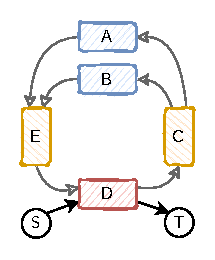
\includegraphics[width=0.85\linewidth]{plasmid_structures/img/plasmid_structure-circular.pdf}
    \caption{Circular}%
    \label{subfig:plasmid_structure:circular}
  \end{subfigure}
  %
  \hfill
  %
  \begin{subfigure}{0.3\linewidth}
    \centering
    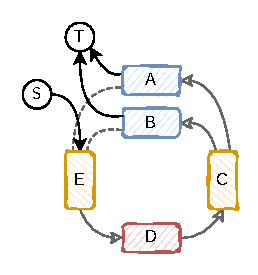
\includegraphics[width=\linewidth]{plasmid_structures/img/plasmid_structure-pc_multi_t.pdf}
    \caption{Partially circular --- multi-\(\mathsf{T}\)}%
    \label{subfig:plasmid_structure:pc_multi_t}
  \end{subfigure}
  %
  \hfill
  %
  \begin{subfigure}{0.3\linewidth}
    \centering
    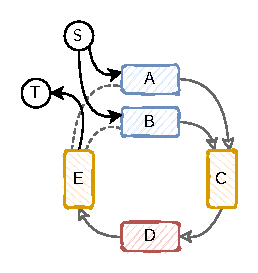
\includegraphics[width=\linewidth]{plasmid_structures/img/plasmid_structure-pc_multi_s.pdf}
    \caption{Partially circular --- multi-\(\mathsf{S}\)}%
    \label{subfig:plasmid_structure:pc_multi_s}
  \end{subfigure}

  \figurecaption{Possible plasmid structures in a sequence graph.}{%
    Let suppose we have a circular plasmid.
    While \subref{subfig:plasmid_structure:circular} gives an instance of the sequence graph where the structure of the plasmid circularity can be found, \subref{subfig:plasmid_structure:pc_multi_t} and \subref{subfig:plasmid_structure:pc_multi_s} give instances where some links are missing, and we cannot satisfy the circularity constraint.
    In each subfigure, the red sequence \(\mathsf{D}\) is a seed, orange and red sequences have a coverage equal to \(2X\) while the blue sequences \(\mathsf{A}\) and \(\mathsf{B}\) have coverage \(X\). In this case, the plasmid contains one repeat composed of sequences \(\mathsf{C}\), \(\mathsf{D}\) and \(\mathsf{E}\).
    For the ease of read, we do not show other links between other plasmids or chromosomes and suppose we cannot merge \(\mathsf{C}\), \(\mathsf{D}\) and \(\mathsf{E}\) in one unitig.
    The links are oriented according to the orientation of the flow.
    %
    \Subref{subfig:plasmid_structure:circular}
    No link is missing.
    To properly model the circularity, the flow through the source-link and the sink-link must equal to zero.
    It is also sufficient to assume one arbitrary orientation of the seed connects either the source and the sink.
    It is thus not necessary to connect the other fragments to the sink.
    The circularity topology and the flow conservation constraints enable to use the full coverage of the plasmid fragments.
    We must constrain on the circularity: for each active oriented fragment, there is at least one incoming link and one outgoing link (without counting the source and the sink links).
    %
    \Subref{subfig:plasmid_structure:pc_multi_t} --- \Subref{subfig:plasmid_structure:pc_multi_s}
    Dashed links are not in the graph.
    If the source must connect a seed, then some sequences are missing in the bin.
    The source should be able to connect several sequences, at the condition that the solution subnetwork graph without \(\mathsf{S}\) and \(\mathsf{T}\) must be connected and contains a seed.
    Also, the active oriented fragments connecting the source cannot have other incoming links.
    Analogously, those connecting the sink cannot have other outgoing links.
  }%
  \label{fig:plasmid_structure}

\end{figure}

The binning flow modelisation in a sequence network graph must be able to:

\begin{itemize}
  \item Find circular bins like in \zcref[S]{subfig:plasmid_structure:circular}:
    \begin{itemize}
      \item We cannot force each flow-arc to be lower-bounded by the total flow if we force the source to connect a seed.
      \item Forcing the source to be connected to a seed, and the sink to be connected to that same seed can be a performance-purpose constraint.
    \end{itemize}
  \item Find partially circular bins like in \zcref[S]{subfig:plasmid_structure:pc_multi_t} and \zcref[S]{subfig:plasmid_structure:pc_multi_s}:
    \begin{itemize}
      \item The source can be connected to any sequence.
      \item The source can be connected to several sequences.
      \item If the source connects a sequence, then there is no other incoming link to that sequence.
      \item Analogously, if the sink connects a sequence, then there is no other outgoing link from that sequence.
      \item The solution subnetwork graph without \(\mathsf{S}\) and \(\mathsf{T}\) must be connected and contain a seed.
    \end{itemize}
\end{itemize}

It is easy to add all the constraints.
The most subtile of them is the last one: we must model an exploration tree containing only one source-arc, and such that each of the network graph arcs can be present in the tree in their original direction, or in their opposite direction.
This problem is defined as the \(ConIntFlow\) problem in this preprint:~\cite{epainMixedIntegerLinear2025}